\newpage
\section{Versionsverwaltung Git}
Git ist eine freie Software zur verteilten Versionsverwaltung von Dateien, die urspr\"unglich f\"ur die Quellcode-Verwaltung des Linux-Kernels entwickelt wurde. Git speichert die Daten nicht auf einen zentralen Server sondern bei jedem User zun\"achst lokal in einem s.g. Repository. So besitzt jeder User den gesamten Code so wie die Versionsgeschichte zun\"achst auf seinem eigenen PC. Ein Remote Repository ist ein Repository das nicht lokal auf dem eigenen Rechner verf\"ugbar ist sondern zentral auf einem Server ausgelagert wird. \"uber einen Push Befehl kann das Remote Repository mit dem lokalem Repository \"uberschrieben werden. Wird ein Fetch Befehl ausgef\"uhrt wird dass Remote Repository mit dem lokalem Repository verglichen und zusammengef\"uhrt (merge Befehl) werden. Im Projekt wurde GitHub, ein webbasierter Hosting-Dienst f\"ur Software-Entwicklungsprojekte verwendet.


\begin{figure}[h]

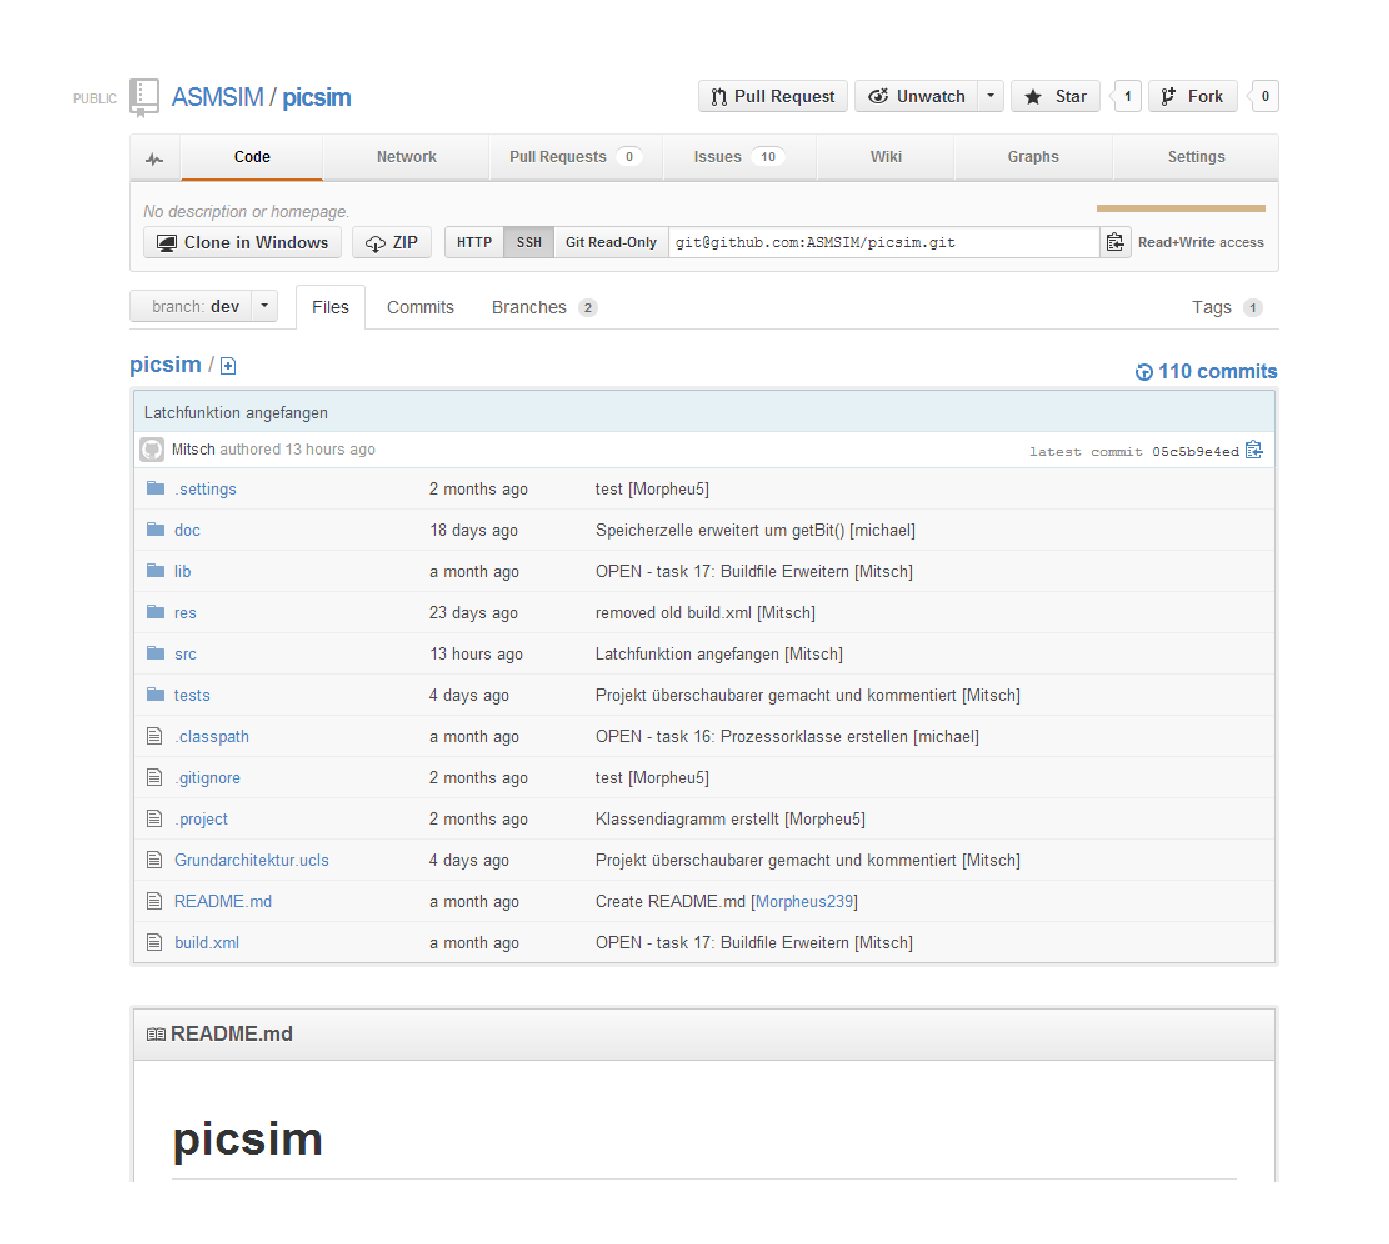
\includegraphics[scale=0.55]{Bilder/Github.pdf}
\caption{Github}
\end{figure}
